\subsection{Import ASTERIX Recording}
\label{sec:ui_import_asterix}

This task allows importing of ASTERIX data recording files into the opened database. \\

\begin{figure}[H]
  \center
    \hspace*{-0.5cm}
    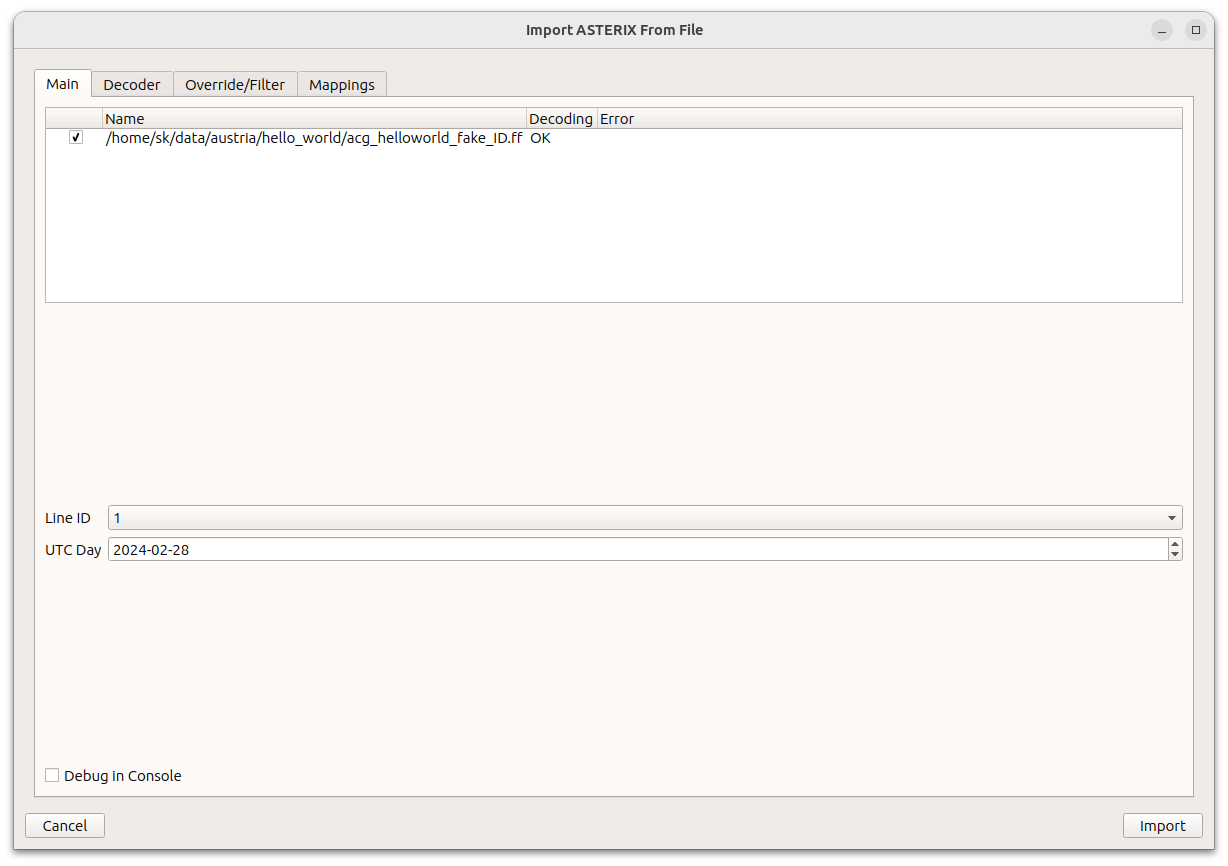
\includegraphics[width=17cm]{figures/asterix_import_data.png}
  \caption{Import ASTERIX data}
\end{figure}

There exist four tabs:

\begin{itemize}
\item Main: File label(s) and status, input line
\item Decoder: jASTERIX decoder settings
\item Override / Filter: Data override settings
\item Mappings: Definition of created database content based on decoded data
\end{itemize}
\ \\

Please \textbf{note} that one or several files can be selected. Since all of the settings are general configuration, please only import several files if they can be imported with the same settings, and do several imports for non-matching files. \\

The following framings are currently supported:

\begin{itemize}
\item Raw/Netto: Unframed ASTERIX data blocks
\item IOSS: IOSS Final Format
\item IOSS\_SEQ: IOSS Final Format with sequence numbers
\item RFF: Comsoft RFF format
\end{itemize}
\ \\

Please \textbf{note} that the following ASTERIX categories, editions, reserved expansion fields and special purpose fields are currently supported: \\

\begin{tabular}{ | l | r | r | r |}
\hline
  CAT & Editions & REFs & SPFs  \\ \hline
  001 & 1.1 &  &  \\ \hline
  002 & 1.0 &  &  \\ \hline
  010 & 0.24 Sensis, 0.31  &  &  \\ \hline
  019 & 1.2, 1.3 & & \\ \hline
  020 & 1.5, 1.8 & 1.3 & \\ \hline
  021 & 0.26, 2.1, 2.4 & 1.5 & \\ \hline
  023 & 1.2 & & \\ \hline
  030 & 7.0 & & \\ \hline
  034 & 1.26 & & \\ \hline
  048 & 1.15, 1.23 & 1.9 & \\ \hline
  062 & 1.12, 1.16, 1.18 & 1.2 & ARTAS TRIs \\ \hline
  063 & 1.0, 1.1 & & \\ \hline
  065 & 1.2, 1.3 & & \\ \hline
  247 & 1.2 & & \\ \hline
  252 & 7.0 & & \\ \hline
\end{tabular} \\
\  \\

Please \textbf{note} that sensor status messages can be decoded, but are not inserted into the database. 
Decoding of ASTERIX CAT002 is recommended if CAT001 data is imported, since the timestamps are derived from it (if not available in CAT001).

\subsubsection{Main Tab}

At the top, the recording files to be imported are shown, with the following items existing for each:
\begin{itemize}
\item Checkbox: Checkbox to indicate if the file should be imported
\item Name: Path and filename
\item Decoding and Error: Indicating possible decoder issues
\end{itemize}
\ \\

Below, the following items exist:
\begin{itemize}
\item Line ID: Line into which all data should be written
\item UTC Day: Date of the recording (for all data)
\item Debug in Console: Additional debugging information is output to the console, and the ASTERIX decoding is switched to single-threading for easier investigation \\
\end{itemize}

\subsubsection{Decoder}

In this tab, all decoder settings can be configured. Please \textbf{note} that changing the settings will trigger a re-evaluation if the recordings can be imported correctly, 
therefore changing the information displayed in the main tab.

\begin{figure}[H]
  \center
    \hspace*{-0.5cm}
    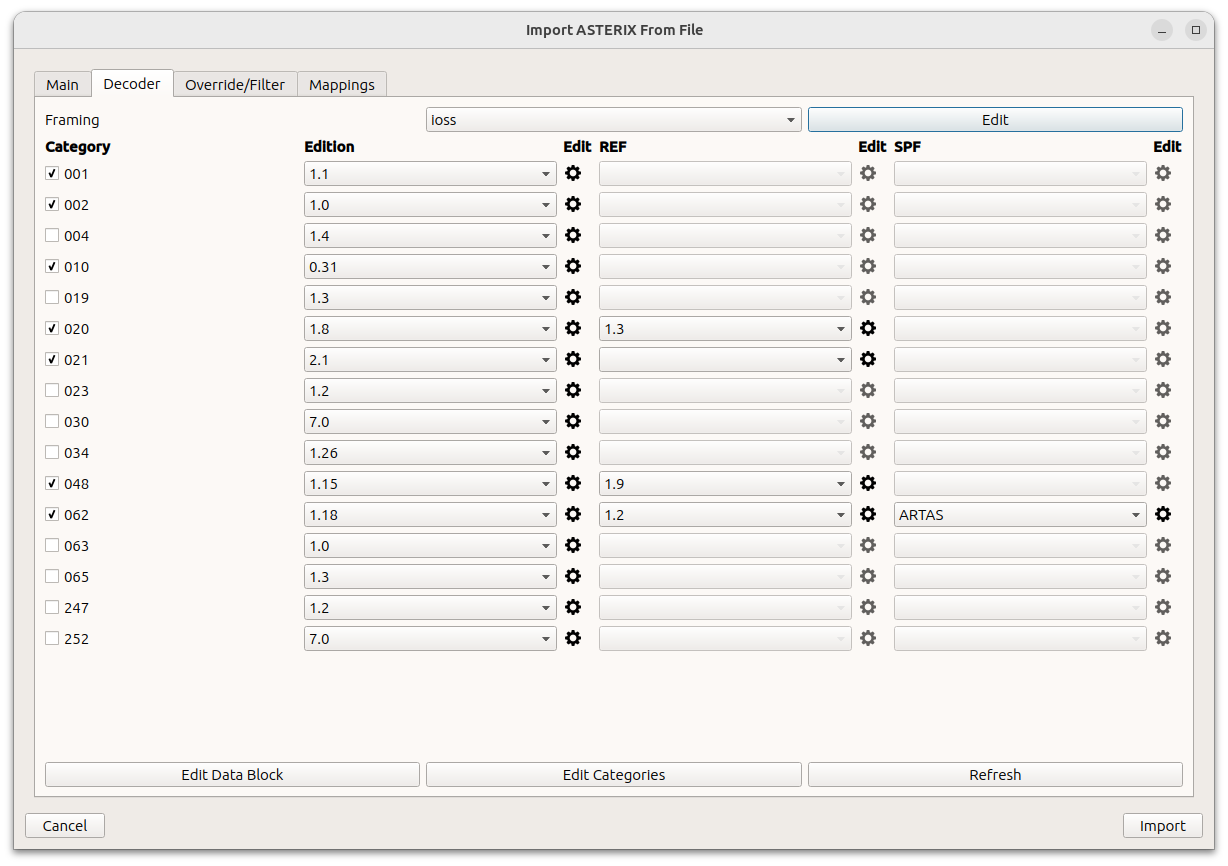
\includegraphics[width=17cm]{figures/asterix_import_data_decoder.png}
  \caption{Import ASTERIX data Decoder}
\end{figure}

\paragraph{Framing}
Using the 'Framing' drop-down menu, the current framing can be selected. Using the 'Edit' button, the current framing definition is opened in a text editor.

\paragraph{Categories}

For each category, a number of elements exist:

\begin{itemize}
\item Category checkbox: Number of category and checkbox defining if it should be decoded
\item Edition: Drop-down menu to select the edition number to be used
\item Edition Edit Button \includegraphics[width=0.5cm]{../../data/icons/edit.png}: Opens the current edition definition in a text editor
\item REF: Drop-down menu to select the Reserved Expansion Field definition (if available)
\item REF Edit Button \includegraphics[width=0.5cm]{../../data/icons/edit.png}: Opens the current REF definition in a text editor
\item SPF: Drop-down menu to select the Special Purpose Field definition (if available)
\item SPF Edit Button \includegraphics[width=0.5cm]{../../data/icons/edit.png}: Opens the current SPF definition in a text editor
\end{itemize}
\ \\

\paragraph{Additional}

Using the 'Edit Data Block' button, the ASTERIX data block definition is opened in a text editor. \\

Using the 'Edit Categories' button, the ASTERIX definitions file is opened in a text editor. \\

Using the 'Refresh' button, all of the jASTERIX definitions are re-loaded from harddisk (e.g. to update after file changes were made). \\

\subsubsection{Override / Filter Tab}
\label{sec:task_import_asterix_override}

\begin{figure}[H]
  \center
    \hspace*{-0.5cm}
    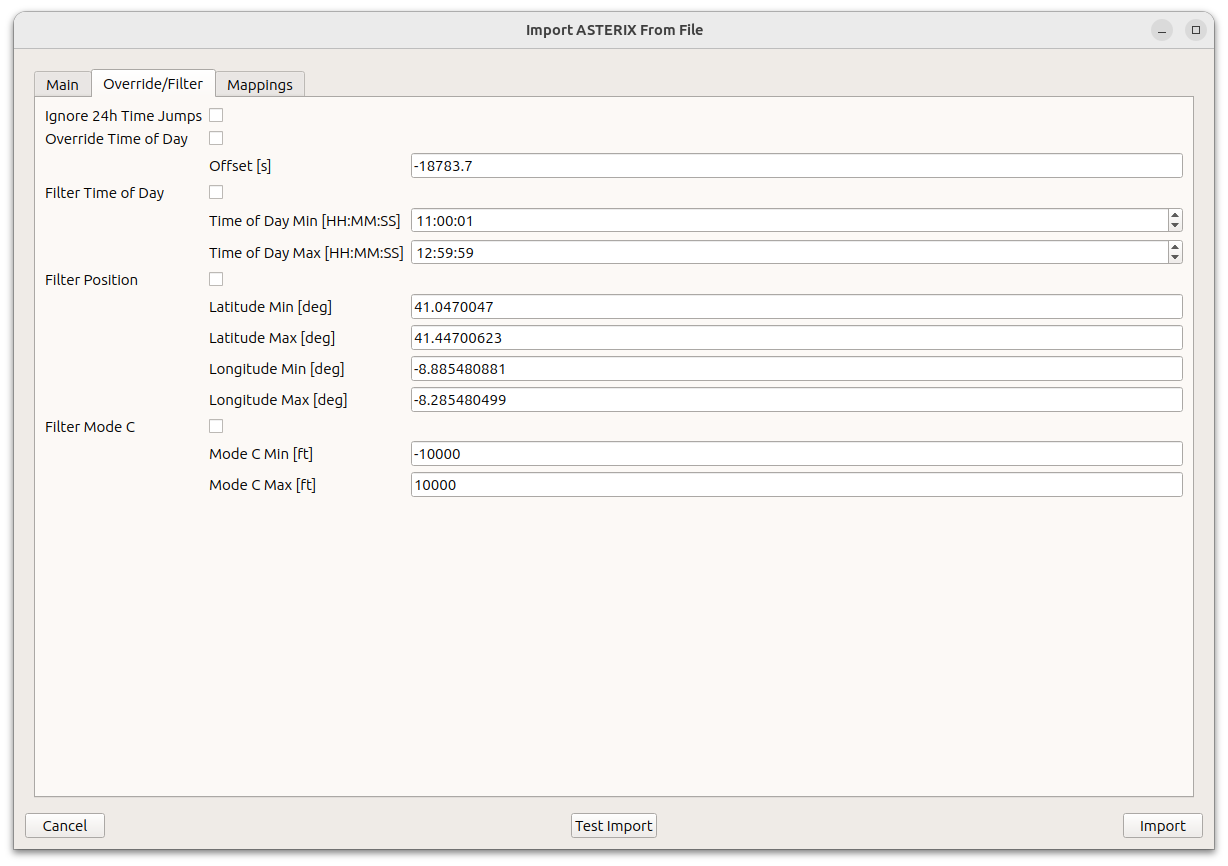
\includegraphics[width=17cm]{figures/asterix_import_data_override.png}
  \caption{Task: Import ASTERIX data Override / Filter}
\end{figure}

These features should only be used in very specific circumstances.

\begin{itemize}
\item Time Correction
\begin{itemize}
\item Ignore 24h Time Jumps: Do not detect 24h time jumps in input data - import everything into same date
\item Override Time of Day: Set offset, which will be added to the 'Time of Day'  item, to correct for unwanted time-shifts
\item Time of Day Offset: Positive or negative offset to be added, in seconds. If the resulting value is out of bounds, it is adjusted to the [0, 86400] interval.
\end{itemize}
\item Filters
\begin{itemize}
\item Filter Time of Day: Use minimum / maximum times, everything outside will be ignored
\item Filter Position: Use minimum / maximum rectangle in latitude and longitude
\item Filter Mode C: Use minimum / maximum rectangle in Mode C. Target reports without Mode C will not be filtered.
\end{itemize}
\end{itemize}
\ \\

Please \textbf{note} that the filtering is applied after the (optional) 'Time of Day' correction is performed. Also, if any filters are active, the import status dialog may not be updated for some time and show wrong time estimates.

\subsubsection{Mappings Tab}

\begin{figure}[H]
  \center
    \hspace*{-0.5cm}
    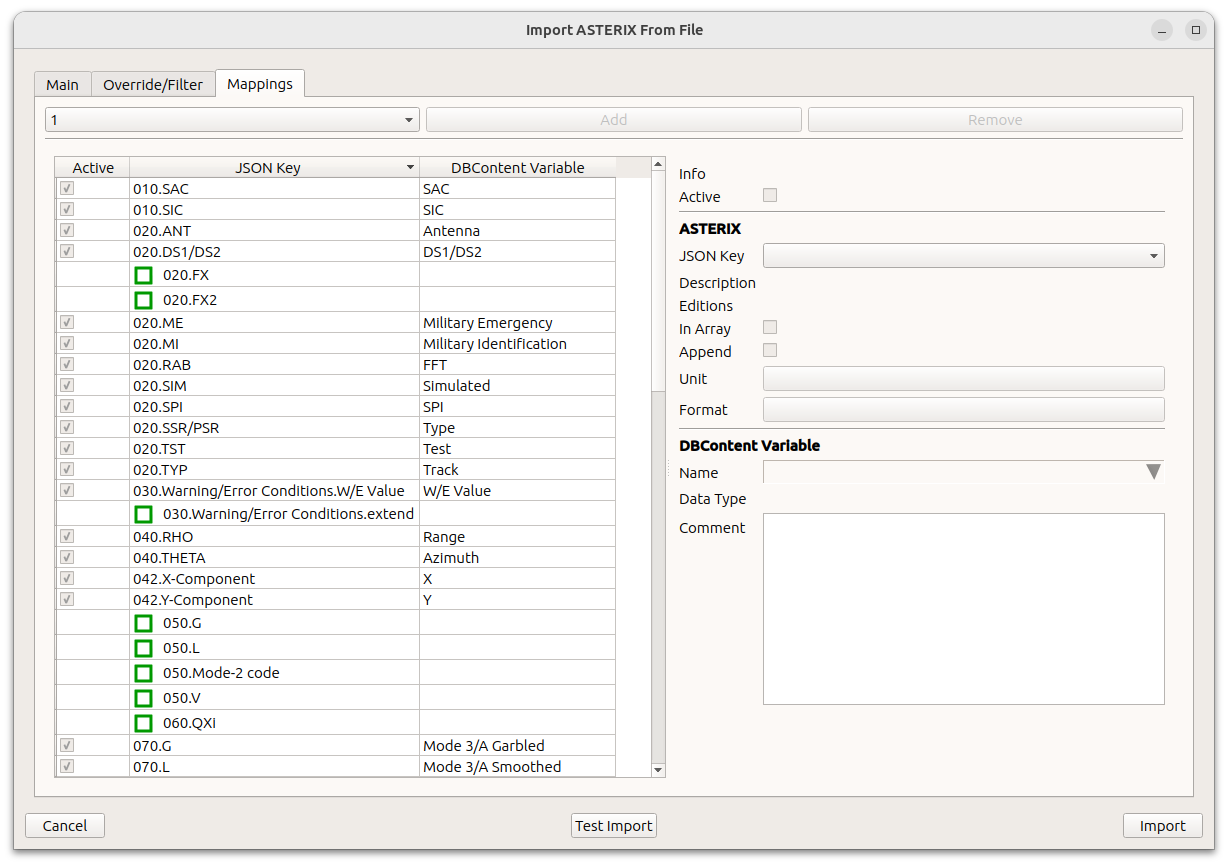
\includegraphics[width=17cm]{figures/asterix_import_data_mappings.png}
  \caption{Task: Import ASTERIX data mappings}
\end{figure}

At the top, the GUI elements can be used to show/add/remove ASTERIX JSON parsers. Below, the currently selected ASTERIX JSON parser is shown and can be configured. \\

An ASTERIX JSON parser in this context is the function that parses the JSON content created by the jASTERIX parser, and creates DBContent from it. 
For each ASTERIX category a dedicated parser defines the mapping from JSON to a DBContent. \\

For the common user interaction is normally not recommended, but sometimes it might be interesting to know what DBContent is created from which ASTERIX data.

\paragraph{Top Elements}

Using the drop-down menu, the to-be-shown parser can be selected. The buttons allow for adding and removing ASTERIX JSON object parsers.

\paragraph{Parser GUI Elements}

The exact definition of how the parsing works is out of scope for this document, so only a short summary is given here. For more information please contact the author.

In the mappings list, the following columns are given:

\begin{itemize}
\item Active checkbox: Defines if the specific mapping is used
\item JSON Key: JSON location and name of the data to be mapped, commonly in 'Data Item Number'.'Variable' or 'Data Item Number'.'Sub Item'.'Variable' format
\item DBContent Variable: Target variable to which this data is mapped
\end{itemize}
\ \\

Whenever a mapping is selected, the details are shown on the right hand side, providing information about the ASTERIX datum (based on the jASTERIX specifications) and the DBContent variable it is mapped to. 
Using the 'Show DBContent Variable' button the variable can be inspected in detail.

\begin{figure}[H]
  \center
    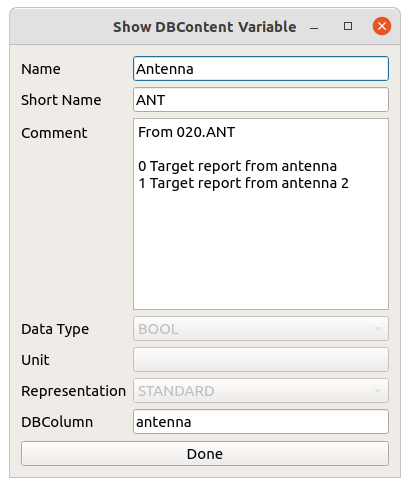
\includegraphics[width=7cm]{figures/asterix_import_data_dbcont_var_details.png}
  \caption{Task: Import ASTERIX Data DBContent Variable Details}
\end{figure}

\subsubsection{Running}

The 'Cancel' button aborts the import.  The 'Import' button triggers the import of the selected files into into the database with the given options, but is only available if all selected files can be decoded correctly. \\

Using the 'Import' button the import task can be performed. During import a status indication will be shown. \\

\begin{figure}[H]
  \center
    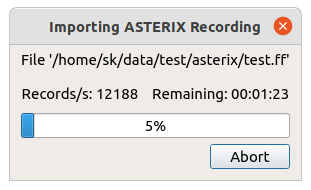
\includegraphics[width=5cm]{figures/asterix_import_data_status.png}
  \caption{Import ASTERIX data status}
\end{figure}

If a decoding error occurs, a brief message box is shown, after which the application has to be closed. 
Please make sure that the correct framing and edition versions are selected, or contact the author for support if this does not resolve the issue. \\

\paragraph{Comments}
The time needed for the import strongly depends on the available CPU performance (multi-threading being very beneficial), but an import of 5 million target reports takes about 3:30 minutes on the author's hardware. \\

The (truncated) timestamps of CAT001 are calculated in a simple algorithm based on the CAT002 messages from the same sensor, so their timestamp data is a bit unreliable, but exact enough for e.g. time window filtering. \\

This task can be run several times, e.g. if multiple ASTERIX recordings from different data sources are to be imported. \\

\includegraphics[width=0.5cm]{../../data/icons/hint.png} Please \textbf{note} the currently not all data fields (as shown in the JSON object parsers) are imported.\\


